\section{Resultados}

Con el archivo con extensión \textit{.l} definido, lo que necesitamos hacer es generar como salida un fichero fuente en C llamado \textbf{lex.yy.c}, para ello hacemos lo siguiente en nuestra terminal:

\begin{lstlisting}
flex lexical.l
\end{lstlisting}

Luego, compilamos el archivo con extensión \textit{.y} para generar los archivos \textit{syntactic.tab.c} y \textit{syntactic.tab.h}:

\begin{lstlisting}
bison -d syntactic.y
\end{lstlisting}

Luego, enlazamos para alimentar de \textit{tokens} al segundo fichero y generar la salida:

\begin{lstlisting}
gcc lex.yy.c syntactic.tab.c -o analyzer -ll
\end{lstlisting}

Una vez el fichero se este ejecutando nosotros podremos probar nuestras definiciones y reglas:

\begin{figure}[H]
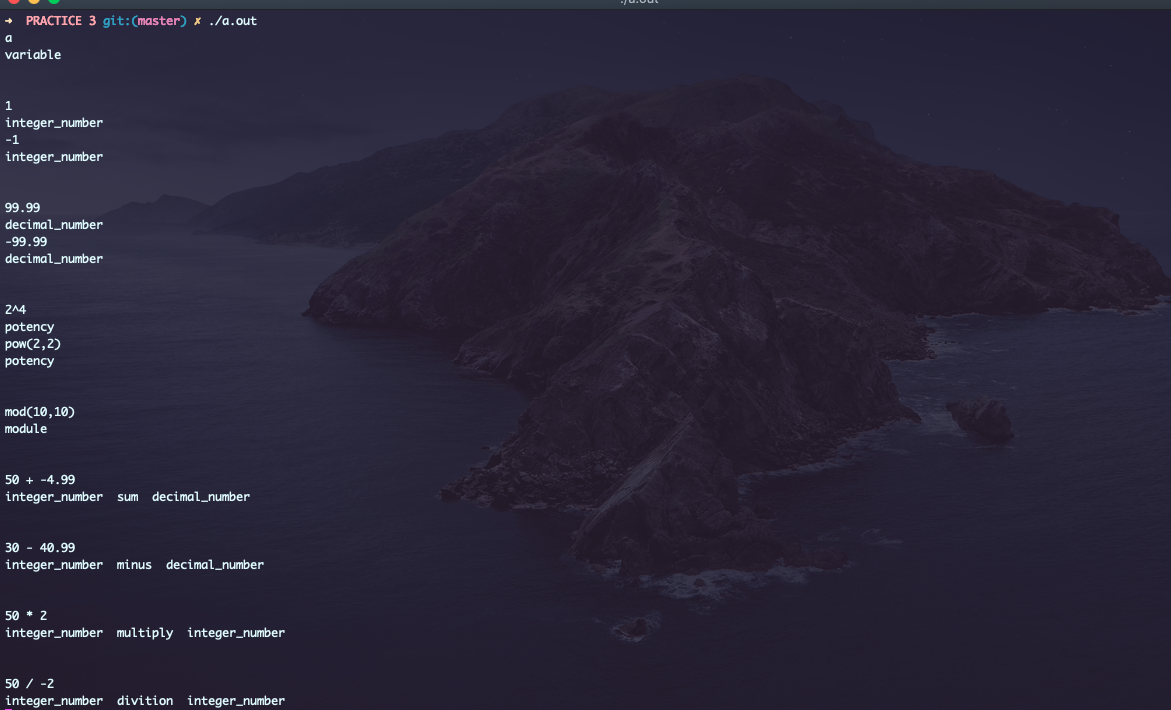
\includegraphics[width = 16.5cm, height = 6cm]{1.png}
\centering \linebreak \linebreak {\small Figure 1.0: Compilación de los programas.}
\end{figure} 

Finalmente, ejecutamos el siguiente comando:

\begin{lstlisting}
./analyzer
\end{lstlisting}

\begin{figure}[H]
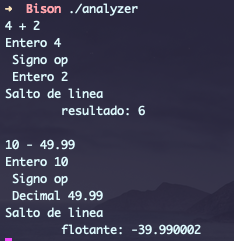
\includegraphics[width = 6cm, height = 8cm]{2.png}
\centering \linebreak \linebreak {\small Figure 2.0: Resultados de las operaciones suma y resta.}
\end{figure} 

\begin{figure}[H]
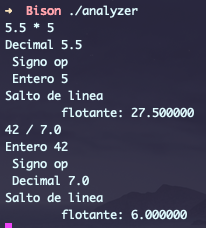
\includegraphics[width = 6cm, height = 8cm]{3.png}
\centering \linebreak \linebreak {\small Figure 3.0: Resultados de las operaciones multiplicación y división.}
\end{figure} 

\begin{figure}[H]
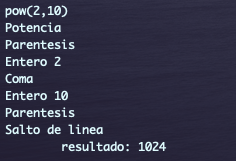
\includegraphics[width = 6cm, height = 8cm]{4.png}
\centering \linebreak \linebreak {\small Figure 4.0: Resultados de la operación potencia.}
\end{figure} 

\pagebreak